\section{Evaluation}
\label{sec:evaluation}

\subsection{Setup}
% Lorenzo's MT-CPA / MT-Dolev experiments (cite opodis-mtrc): n = 100, three families,
% k = 3, 5, 7, t = 1..2k-1, t_s + t_l = k - 1. Abstract: 1000 rounds. Concrete: 2 s window.
% Machine: Intel Core Ultra 5 228V, 8 cores, 30 GB RAM, Fedora, GCC 16.2.1.
\todo{Experimental setup}

\subsection{Correctness}
% Within bounds (f <= min(t_s, t_l); CPA only on "both" networks), no time limits:
% every run must reach 100% liveness and safety.
\todo{Within-bounds check results}

\subsection{Abstract vs Concrete on one machine}
% Figures 2 and 3 of the MT paper on Abstract and BoostMq; run times.
\todo{Fidelity results and run times}

\begin{figure*}
  \centering
  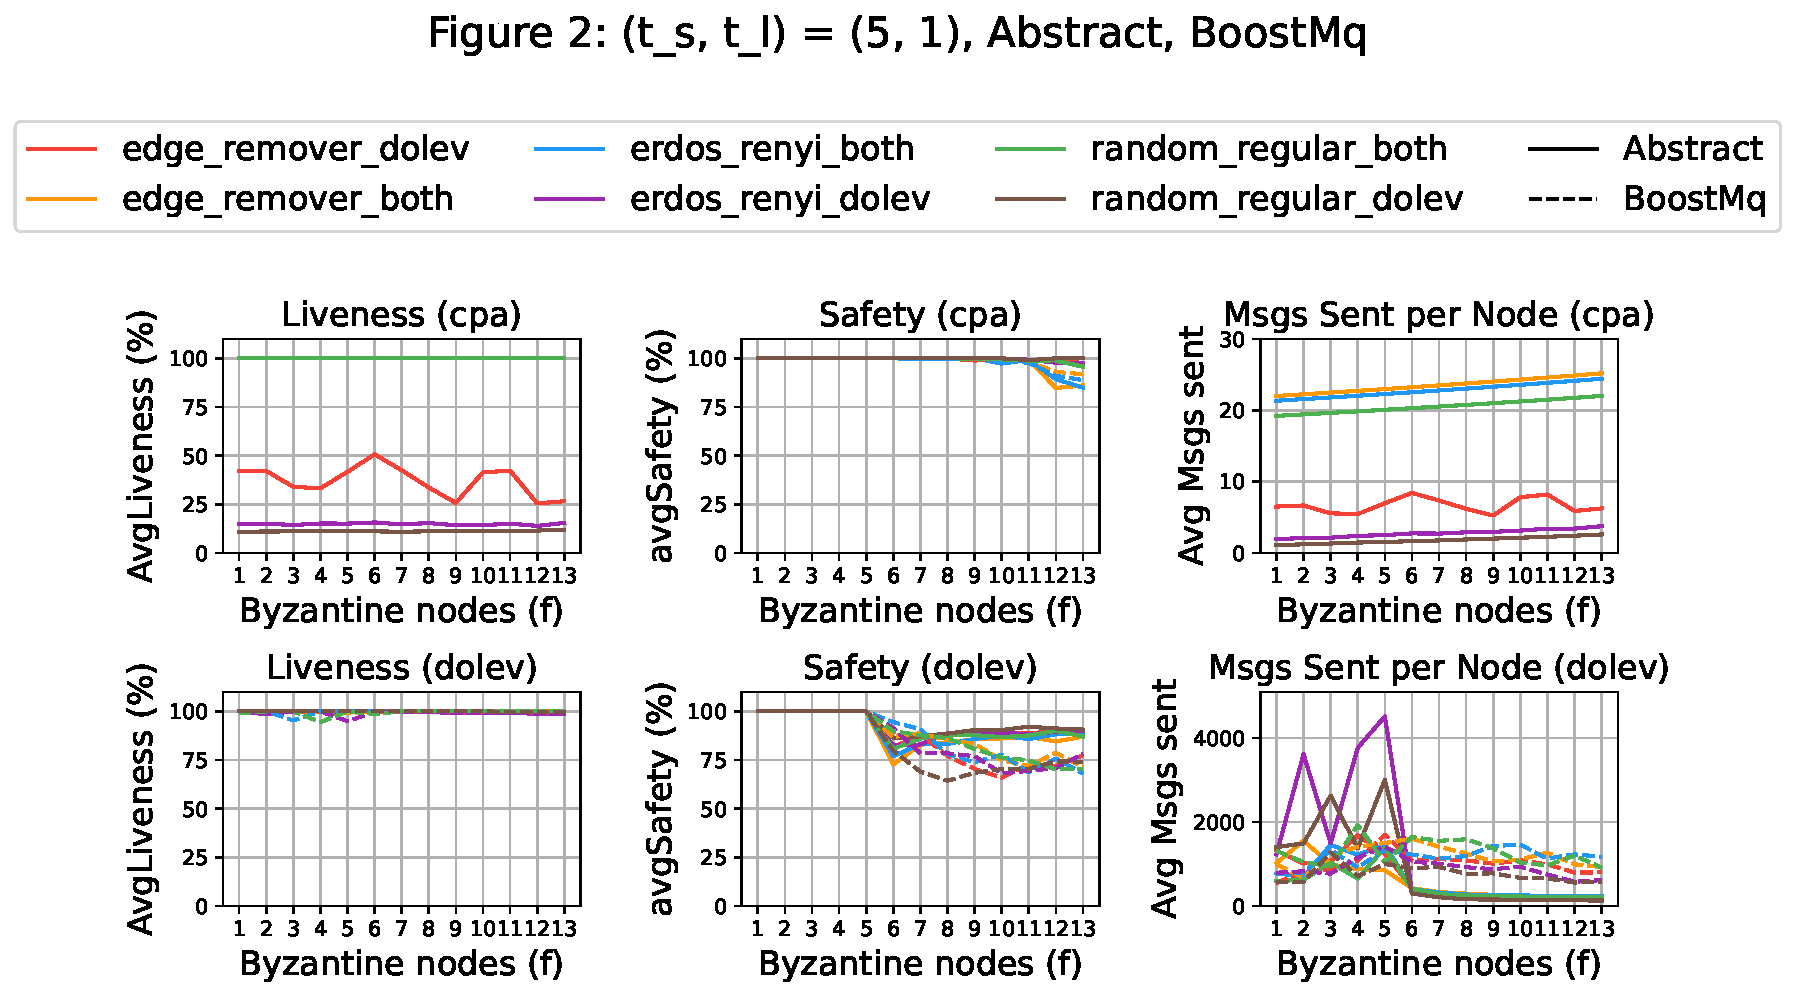
\includegraphics[width=\textwidth]{figures/figure2_combined.pdf}
  \caption{\todo{Caption: $k = 7$, $(t_s, t_l) = (5, 1)$}}
  \label{fig:figure2}
\end{figure*}

\begin{figure*}
  \centering
  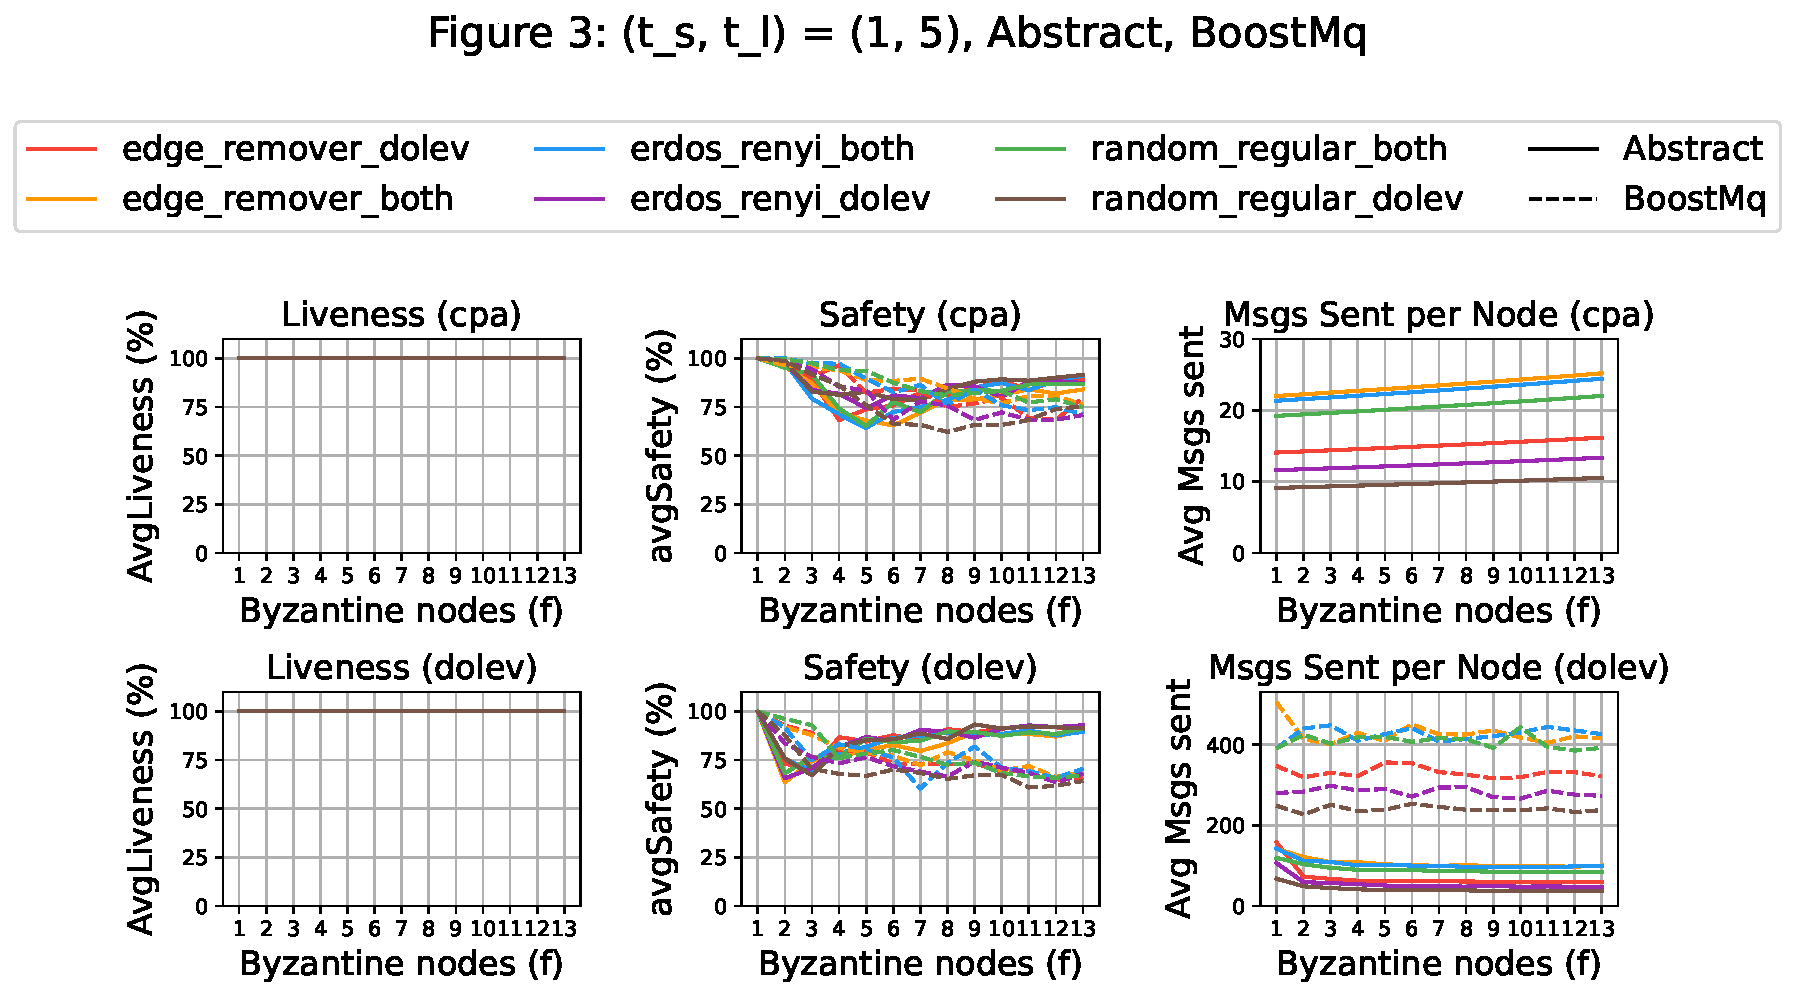
\includegraphics[width=\textwidth]{figures/figure3_combined.pdf}
  \caption{\todo{Caption: $k = 7$, $(t_s, t_l) = (1, 5)$}}
  \label{fig:figure3}
\end{figure*}

\subsection{ZeroMQ on a cluster}
% Bridge: ZeroMQ matches BoostMq on one machine. Then LIP6 cluster: 1 machine x 20 peers,
% 2 machines x 10 peers over tcp://.
\todo{Cluster results}
